\documentclass{article}
\usepackage{natbib}
\usepackage[francais]{babel}
\usepackage[utf8]{inputenc}
\usepackage[T1]{fontenc}
\usepackage{hyperref}
\usepackage{graphicx}
\usepackage{minted}
\usepackage{uqac}
\usepackage{sectioncompilation}

% ================================ Meta data (pour titre et autre)
\discipline{8INF844}
\supervisor{Abdenour Bouzouane}
\project{TP1}
\title{Simulation multi-agents avec NetLogo}
\author{Sébastien Blin\\Victor Drouin Viallard}

% ================================ Document
\begin{document}

\maketitle

\section{Synthèse de l'article}
\subsection{Introduction}
L'article \emph{Flocks, Herds, and Schools: A Distributed Behavioral Model} (\emph{Craig W. Reynolds}) décrit comment simuler des flocks en considérant chaque individu à part, sans avoir à scripter le mouvement de chaque individu, mais plutôt en fonction de l'environnement perçu par ceux-ci. Le flock sera ainsi le résultat du mouvement de chaque individu. À première vue, la simulation d'un flock peut paraître difficile, car il y a beaucoup d'individus à simuler et très dur à maintenir (éviter les collisions entre toutes les particules à chaque frame par exemple), mais ce papier propose une méthode pour réussir à simuler ce mouvement sans avoir à réaliser la gestion des collisions. Ainsi, Le flock sera le résultat du mouvement d'un seul individu appliqué à tous les oiseaux.

On considère ici le flock comme un ensemble de particules améliorées (\emph{boid}). Chaque particule représente un individu (ici un oiseau) et possède des variables (couleur, localisation, velocité, etc) auxquelles on donne une forme (qui est plus significative visuellement et ajoute la notion d'orientation) ainsi qu'une vitesse maximale.

\subsection{Fonctionnement de l'algorithme}
Les observations montre que certains animaux se regroupent en flock afin de se protéger des prédateurs, chercher de la nourriture, etc. Pour participer à un flock, un oiseau doit pouvoir se coordoner avec les oiseaux qui l'entourent. Vu qu'un flock est possiblement infini en taille (certains bancs de poissons ont des millions d'individus), on suppose que l'animal ne considère que lui-même, quelques uns de ses voisins et l'ensemble du flock. On peut alors considérer trois forces~:

\begin{itemize}
  \item \emph{Collision Avoidance}, pour éviter de rentrer en collision avec les autres oiseaux.
  \item \emph{Velocity Matching} (heading + speed => vecteur direction), pour rester à la vitesse des oiseaux voisins.
  \item \emph{Flock Centering}, pour rester proche des oiseaux voisins et aller vers le centre du flock car y a la meme densité partout autour de lui.
\end{itemize}

On observe donc deux forces opposées~: l'une qui pousse l'oiseau à rester dans le flock, l'autre qui le pousse à éviter les autres oiseaux~; il faut y prêter attention car cela peut amener l'oiseau à ne pas savoir où se déplacer.
Les trois forces agissent indépendament et propose une solution différente au choix de la direction à prendre. On peut alors décider d'atténuer plus ou moins telle ou telle force et les combiner pour obtenir le mouvement résultant des 3 forces, etc. Si moyenner ces trois forces est la solution la plus simple, Il semble plus intéressant de les prioritiser puis de les accumuler dans l'ordre jusqu'à atteindre une magnitude totale maximale, pour éviter les problèmes d'opposition évoqués précédemment. Par exemple, si on regarde en priorité la force de \emph{Collision Avoidance} et qu'elle est de magnitude plus forte que celle maximale alors on suivra directement cette force pour éviter en priorité la collision et les autres forces seront temporairement écartées.

\subsection{Améliorations possibles}
On peut enfin ajouter des fonctionnalités comme l'initialisation de la position des obstacles, des oiseaux ou encore leur donner un but de migration au fur et à mesure. La plus intéressante des fonctionnalité est l'évitement d'objets. Pour la réaliser, deux solutions sont envisageables. La première, \emph{force field concept}, consiste à avoir une force de répulsion autour de l'objet à éviter, mais si l'oiseau arrive pile en face d'une ligne du champ, il ne sera pas repoussé mais ralenti jusqu'à se bloquer. De plus, si l'oiseau vole à coté d'un mur il n'a pas besoin de tourner même s'il est dans le champ, ce qui nous amène à la seconde, \emph{steer-to-avoid}, où l'oiseau ne considère que les obstables face à lui. S'il en trouve un, il calcule alors un vecteur afin d'éviter l'objet.

\subsection{Conclusion}
On peut trouver plusieurs applications concrètes à la simulation d'un flocking, par exemple dans la simulation de traffics routiers ou encore pour l'observation d'animaux.
Enfin, il est possible d'améliorer l'algorithme en le parrallélisant ou en étant sûr que $N$ soit assez petit (en considérant seulement une partie du flock par exemple).

\section{Modification du code source}

Le Flock se base donc sur 3 forces, séparées en 3 fonctions dans le code~:
\begin{itemize}
  \item \emph{separate [turtlesaround]}, pour empêcher que les turtles rentrent en contact. Ici, un vecteur force est calculé entre une turtle et les voisins qu'elle détecte. Ce vecteur est alors pondéré par la distance entre les deux turtles. Ainsi, plus les turtles sont proches, plus la force de séparation sera forte.
  \begin{figure}[h]
  	\begin{center}
  		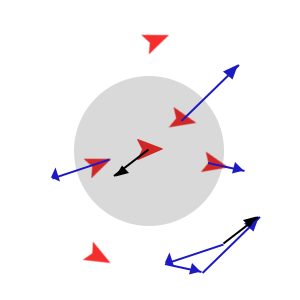
\includegraphics[scale=0.3]{img/separate}
  		\caption{Force de séparation}
  		\label{fig:separate}
  	\end{center}
  \end{figure}
  \item \emph{align [turtlesaround]}, qui sert à aligner les turtles dans la même direction. Ici on prend les vecteurs d'alignement de chaque turtle, et on considère le vecteur moyen.
  \begin{figure}[h]
  	\begin{center}
  		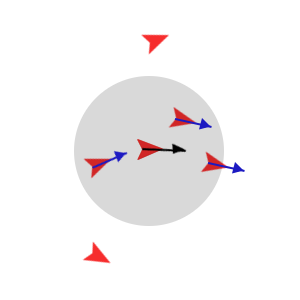
\includegraphics[scale=0.3]{img/align}
  		\caption{Force d'alignement}
  		\label{fig:align}
  	\end{center}
  \end{figure}
  \item \emph{cohere [turtlesaround]} qui résulte en un vecteur pour diriger la turtle vers le centre de gravité de ses voisins.
  \begin{figure}[h]
  	\begin{center}
  		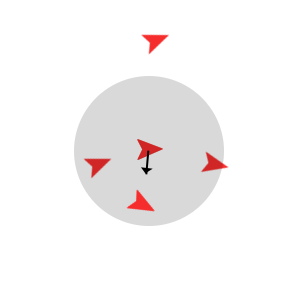
\includegraphics[scale=0.3]{img/cohere}
  		\caption{Force de cohésion}
  		\label{fig:cohere}
  	\end{center}
  \end{figure}
\end{itemize}

\section{Ramassage d'objets}

De plus, nous pouvons générer des objets aléatoires sur le terrain. Les oiseaux peuvent alors prendre ces objets et le lacher lorsqu'un objet du même type se situe à côté de ce point. Un oiseau ne peut pas prendre plusieurs objets. L'idée est donc de former des tas avec les objets générés.
2 scénarios ont été réalisés (cf plus loin). Soit l'agent récupère un objet et le garde jusqu'à la fin, soit il peut le lacher afin de former des tas.

\section{Pondération des forces}

Nous avons tenté plusieurs scénarios et nous obtenons un résultat qui fonctionne avec la configuration suivante~:
\begin{itemize}
  \item population 200
  \item align-factor 5,75
  \item cohere-factor 0,4
  \item separate-factor 2,0 (minimum separation 2,5 et une vision de 8 patches)
\end{itemize}
On remarque que la force de cohésion est plus forte que les deux autres forces, on la multiplie donc par un facteur faible.

\section{Mesure de performance}

Afin de mesurer la performance du flock, nous avons décider de mesurer le nombre de voisins détectés par la $turtle 0$. Ainsi, si le flock fonctionne, le nombre de voisin devrait augmenter.

\begin{figure}[h]
	\begin{center}
		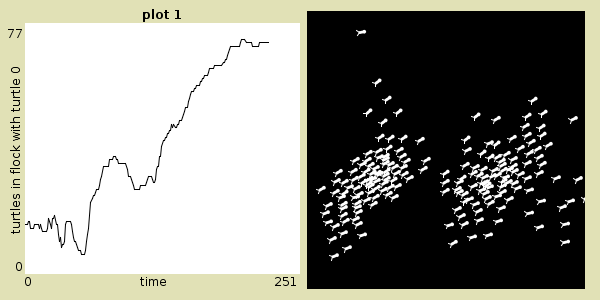
\includegraphics[scale=0.5]{img/performance}
		\caption{Performance avec les pondérations données précédement}
		\label{fig:performance}
	\end{center}
\end{figure}

\section{Pondération d'un non-flock}
De plus, si la force de cohésion est nulle, les agents ne se comporteront plus en flock, peu importe les valeurs des deux autres forces et le ramassage d'objets pour en faire des tas est beaucoup plus lent (mais continue de fonctionner car les agents reste en général dans la même direction).

\section{Création de tas}

Pour cette question, nous avons désactivé les drop d'objets. Ainsi, lorsqu'un oiseau prend un objet il le garde jusqu'à la fin.
Les forces ont été modifiés de sorte à~:
\begin{itemize}
  \item La force de séparation est plus forte (d'un facteur 10) si l'agent n'est pas de la même couleur
  \item La force d'alignement ne s'aligne qu'avec les agents possédant les mêmes objets
  \item Le force de cohésion ne se fait qu'avec les agents possédant le même objet
\end{itemize}
On commence à voir des groupes se former avec les paramètres ci-dessus au bout de 2000 ticks.
\section{Interface}
\begin{figure}[h]
	\begin{center}
		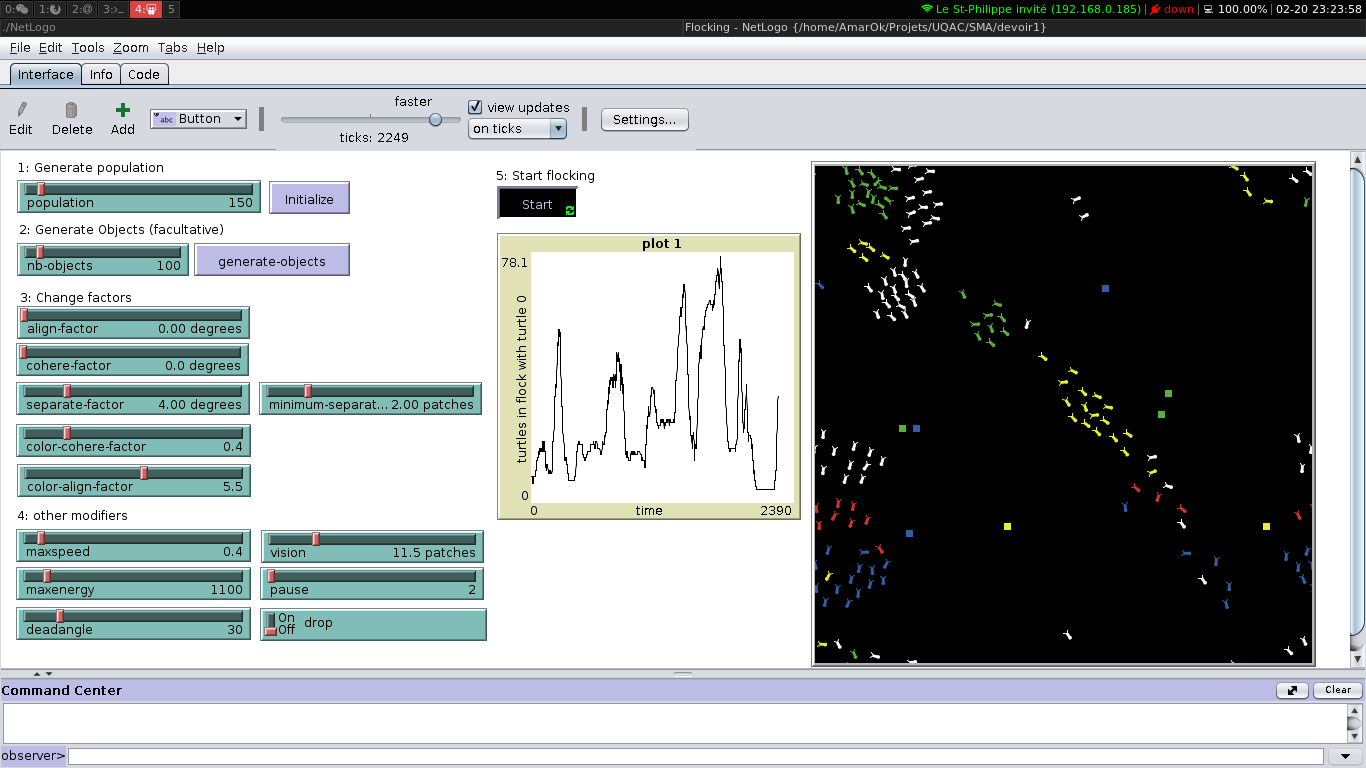
\includegraphics[scale=0.3]{img/groups}
		\caption{Des groupes de flocks}
		\label{fig:groups}
	\end{center}
\end{figure}

\section{Comparaison des 2 flocks}
Au final, outre le fait que l'exemple de flocking de NetLogo soit plus basique (pas de gestion de récupération d'objet, d'énergie, de formations de tas, etc. La séparation du modèle précédent ne se base que sur le voisin le plus proche, ce qui fait qu'un agent rebondi dans le cas où l'agent possède un voisin de chaque côté alors qu'avec notre modèle, l'agent restera environ entre les deux agents. Le mouvement sera donc plus naturel.
De plus, le fait de limiter le mouvement avec une limite de degrés (pour les forces de cohésion et d'alignement n'est pas forcément pertinent d'un point de vue naturel, un oiseau pouvant généralement changer de direction relativement rapidement). Cependant, il possède pour avantage d'être simple et peu gourmand en calculs pour NetLogo.

\section{Ajout de fonctionnalités}

Deux fonctionnalités ont été ajoutées. La première est la consommation d'énergie. Chaque agent possède un niveau d'énergie entre 1 et $maxenergy$. Cette charge baisse de 1 par tick. Une fois que l'agent n'a plus d'énergie, il s'arrête, lâche l'objet s'il en possède un et se met en pause. Il possède ensuite $1/pause$ probabilité de repartir à chaque tick. Au départ, il choisit d'une nouvelle direction.

La seconde fonctionnalité est le champ de vision. L'agent possède un angle mort à l'arrière qui est paramétrable avec une valeur entre 0 et 180. Par exemple, lorsque cette valeur est paramétrée à 30°, l'agent possède donc un angle mort de 60° à l'arrière. Si un autre agent se trouve dans cet angle, il est ignoré.

\section{Interface}
\begin{figure}[h]
	\begin{center}
		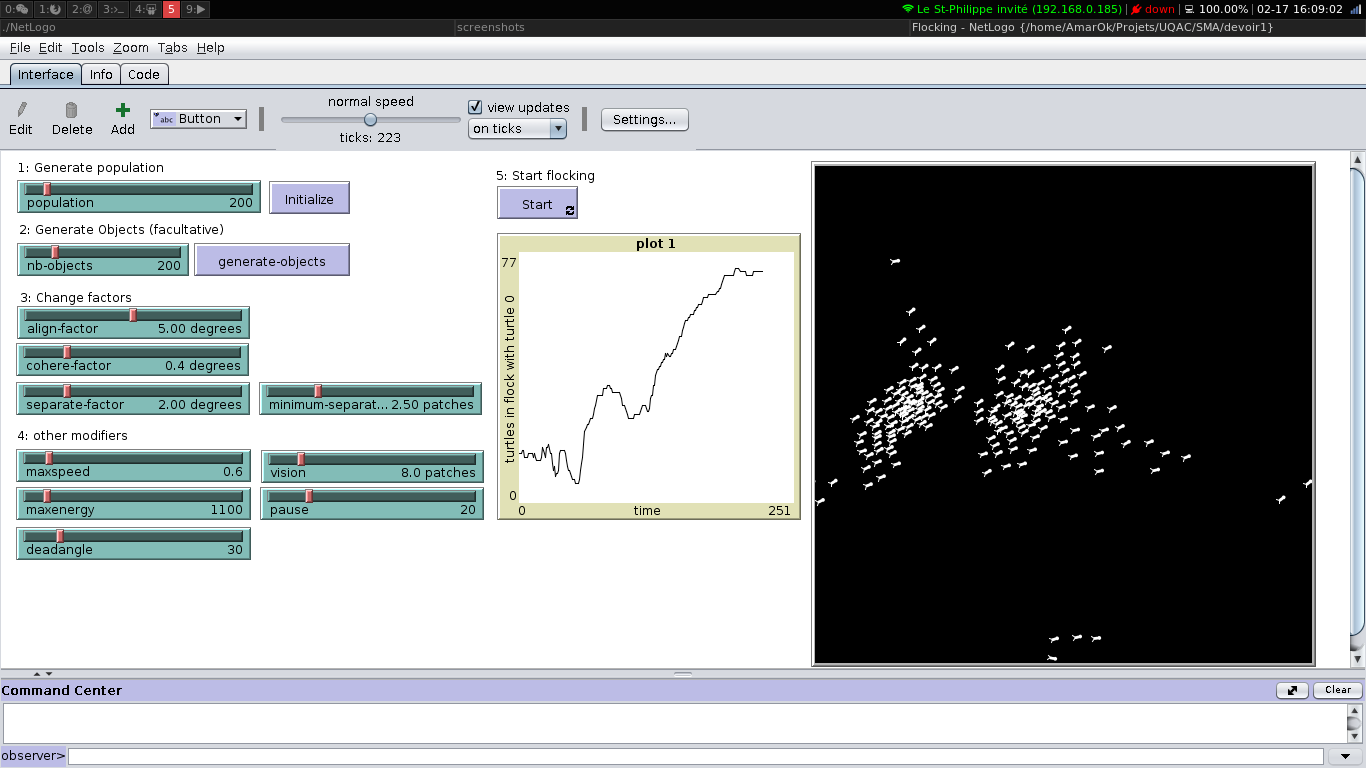
\includegraphics[scale=0.3]{img/interface}
		\caption{Interface finale}
		\label{fig:interface}
	\end{center}
\end{figure}

\end{document}
